\chapter{Results}
\label{chap:Results}
\paragraph*{}
From the design given in the previous chapter \ref{chap:theory}, two implementations are created. One without scanline buffers, and the other with scanline buffering. In the following sections, the results from the simulations, synthesis and hardware testing of theses implementations will be presented and discussed. \\
To ensure that the generated results are correct, a Matlab verification script is created (appendix \ref{app:Matlab}). The script contains a reference calculation of the Sobel filter, that mimics the expected and desired operation of the VHDL implementation.
The calculated reference, is subsequently compared with the output image generated by either the simulation or the hardware test.

\textcolor{red}{resource usage slices, LUT's ??}
\section{Implementation of Sobel operator without scanline buffering.}
\paragraph*{}
With the design given in the ASM diagram (figure \ref{fig:ASM_HW} in section \ref{sec:AccDesign}, the VHDL source found in appendix \ref{app:acc2} has been implemented. The implementation have been synthesised, simulated and tested on the \textit{Nexys3 board} and the result is successfully verified by the Matlab verification script.\\
Figure \ref{fig:sum_synthesis_report}, shows an extract from the synthesis report that is generated by the \textit{Xilinx  ISE tool}. The number of inferred D-flip flops are identical to the anticipated values given in table  \ref{tab:designRegisters} and table \ref{tab:designAdders} and the number of adders are two more than the expected number. This discrepancy might be caused by the absolute (\textit{abs()}) functions, which could be constructed from a multiplexer and an adder. 

\begin{figure}[H]
\centering
\small
\begin{BVerbatim}
Summary:
    inferred  31 Adder/Subtractor(s).
    inferred 232 D-type flip-flop(s).
    inferred   3 Comparator(s).
    inferred  59 Multiplexer(s).
    inferred   1 Finite State Machine(s).
\end{BVerbatim}
\caption{Summary of synthesis report ISE project navigator}
\label{fig:sum_synthesis_report}
\end{figure}

From the post place and route report, the maximum frequency is shown in figure \ref{fig:sum_PostPAR_report}. The limiting factor is assumed to by combinatorial circuit that performs the Sobel filter calculation of the sliding window. 

\begin{figure}[H]
\centering
\small
\begin{BVerbatim}
Timing summary:
---------------
Design statistics:
   Minimum period:   9.729ns   (Maximum frequency: 102.785MHz)
\end{BVerbatim}
\caption{Post place and route timing summary.}
\label{fig:sum_PostPAR_report}
\end{figure}

\paragraph*{}
During the implementation and verification of the design, simulations have been performed in ModelSim. Simulations are applied on an image of a roller coaster with an image dimension of $352x288$ pixels, see figure \ref{fig:test_picture_raw}. The image is supplied as part of lab assignment \cite{Sparsoe2014}. The output image from the simulation is seen in figure \ref{fig:test_picture_sobel} and it has been successfully validated by the MATLAB verification script.

\begin{figure}[H]
	\centering
	\begin{subfigure}[b]{0.4\textwidth}
		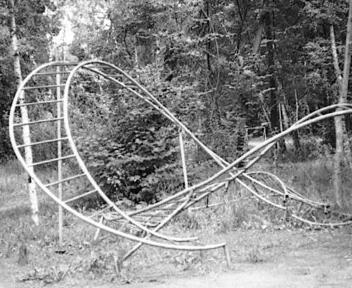
\includegraphics[width=1 \textwidth]{raw.png}
		\caption{Original image before simulation}
		\label{fig:test_picture_raw}
    \end{subfigure}%
        ~ %add desired spacing between images, e. g. ~, \quad, \qquad, \hfill etc. 
    \begin{subfigure}[b]{0.4\textwidth}
    	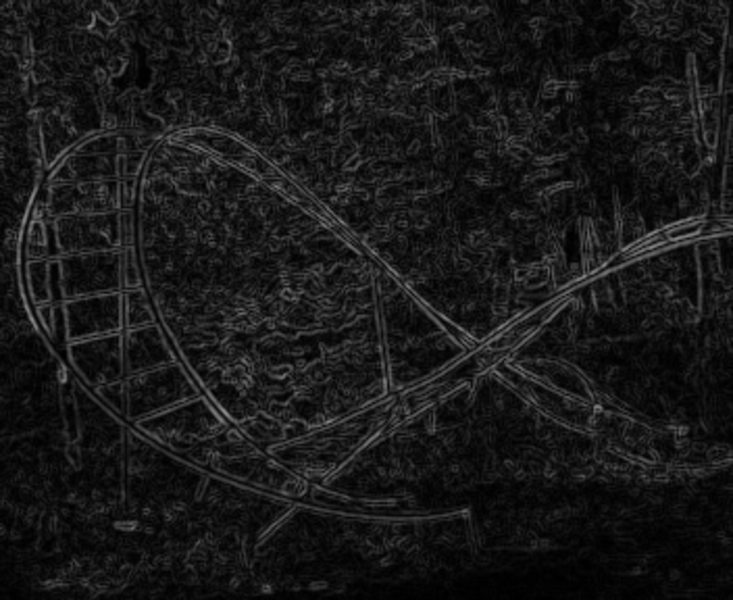
\includegraphics[width=1 \textwidth]{sobel_result.pdf}
    	\caption{Sobel image from simulation}
    	\label{fig:test_picture_sobel}
	\end{subfigure}
	\caption{Simulation result of basic design}
\end{figure}

\paragraph*{}
The simulation is completed in $24.4ms$ which results in a throughput of $40.9$ $frames~pr.~sec$ or $4.15Mpix/sec$, this is in accordance with the estimate done in section \ref{sec:AccDesign}. A part of the simulation waveform can be seen in figure \ref{fig:acc2_waveform}. The waveform depicts one full cycle (6 clock cycles) used when processing a pixel pair. The waveform is annotated to show how the sliding window is shifted, during the state \emph{readSetup} and filled with incoming pixel pairs in the three subsequent states (\emph{readCenter}, \emph{readAbove} and \emph{readBelow}). Finally it shows the result (\emph{dataW}) being written to the output image at an offset memory location (\emph{addr}).

\begin{figure}[H]
	\centering
    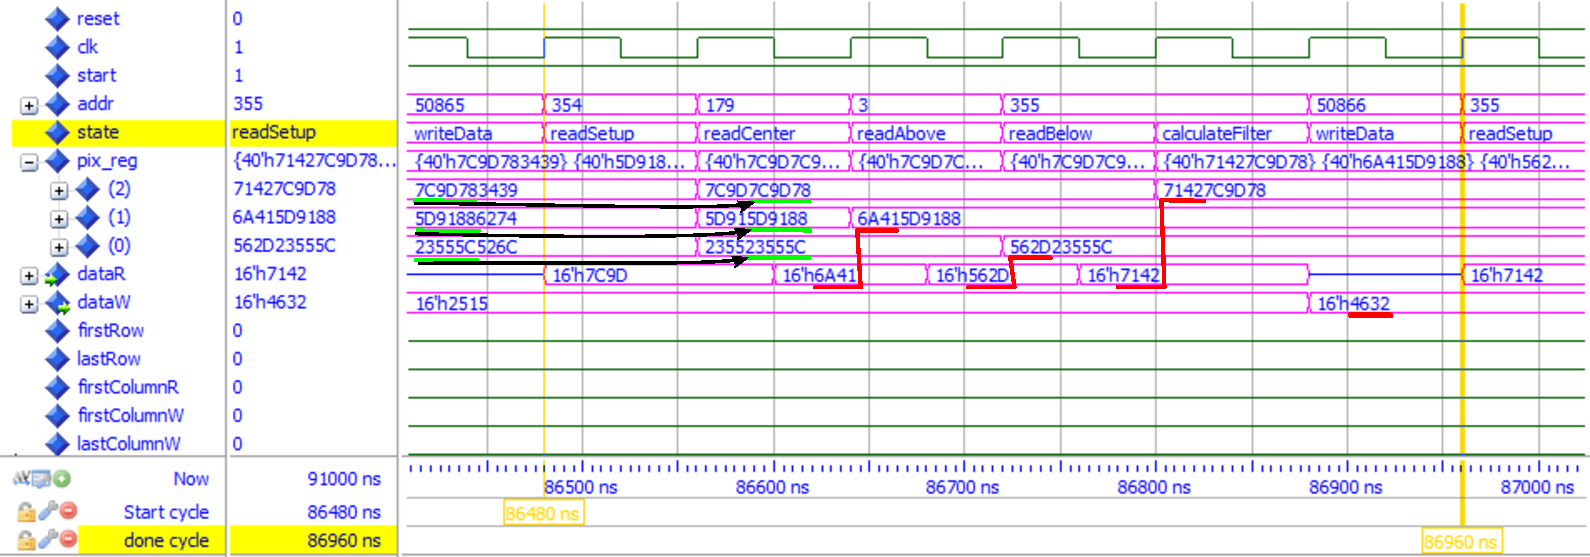
\includegraphics[width=1 \textwidth]{acc2_annotated.pdf}
	\caption{Simulation waveform}
	\label{fig:acc2_waveform}
\end{figure}


\section{Optimization with scanline buffers}
\paragraph*{}
In section \ref{sec:Optimization} a design using scanline buffering was described. This scanline based design has been implemented and synthesized, the results from the simulations and hardware tests have passed the verification script. The VHDL implementation is found in appendix \ref{app:accScanline}. \\
Because this design is using the same circuits for the Sobel calculation and the sliding window, the synthesis report gives roughly the same amount of logic components, See figure \ref{fig:sum_synthesis_report_scan}.
In the synthesis report it is also possible to locate the two dual port block RAM components that is used to form the three scanline buffers. Figure \ref{fig:sum_synthesis_report_ram} list the two inferred block RAMs components. The VHDL implementation of the block RAM can be found in appendix \ref{app:bram}.
    
\begin{figure}[H]
\centering
\small
\begin{BVerbatim}
Summary:
    inferred  34 Adder/Subtractor(s).
    inferred 230 D-type flip-flop(s).
    inferred   5 Comparator(s).
    inferred  75 Multiplexer(s).
    inferred   1 Finite State Machine(s).
\end{BVerbatim}
\caption{Summary of the synthesis report}
\label{fig:sum_synthesis_report_scan}
\end{figure}

\begin{figure}[H]
\centering
\small
\begin{BVerbatim}
Synthesizing Unit <bram_tdp_1>.
    Related source file is "\bram_tdp.vhd".
        DATA_WIDTH = 16
        ADDR_WIDTH = 9
    Found 512x16-bit dual-port RAM <Mram_mem> for signal <mem>.
    Found 16-bit register for signal <b_dout>.
    Found 16-bit register for signal <a_dout>.
    Summary:
	inferred   1 RAM(s).
	inferred  32 D-type flip-flop(s).
Unit <bram_tdp_1> synthesized.

Synthesizing Unit <bram_tdp_2>.
    Related source file is "\bram_tdp.vhd".
        DATA_WIDTH = 16
        ADDR_WIDTH = 8
    Found 256x16-bit dual-port RAM <Mram_mem> for signal <mem>.
    Found 16-bit register for signal <b_dout>.
    Found 16-bit register for signal <a_dout>.
    Summary:
	inferred   1 RAM(s).
	inferred  32 D-type flip-flop(s).
Unit <bram_tdp_2> synthesized.
\end{BVerbatim}
\caption{Inferred Block RAM (synthesis report)}
\label{fig:sum_synthesis_report_ram}
\end{figure}

The maximum clock rate is decreased slightly as seen in figure \ref{fig:sum_ScanPostPAR_report} - A little surprisingly, considering that the combinatorial logic for the Sobel filter is identical to the previos design. One possible explanation, is that the introduction of the block RAMs requires a different place and route layout with longer traces to the output pins (eg. data bus to external RAM).
%I don't think this is reason: The fact that the entire sliding window is updated in one clock cycle, means that the longest combinatorial path for Sobel calculation becomes slighly longer. In the previous design the only one line was updated at a time ...

\begin{figure}[H]
\centering
\small
\begin{BVerbatim}
Timing summary:
---------------
Design statistics:
   Minimum period:  11.134ns   (Maximum frequency:  89.815MHz)
\end{BVerbatim}
\caption{Post place and route timing summary.}
\label{fig:sum_ScanPostPAR_report}
\end{figure}

\paragraph*{}
The simulation of the optimized implementation shows, that by using the scanline buffering described in section \ref{sec:Optimization}, we have managed to reduce the number of memory transactions to the absolute minimum - pixels are only touched once. This is witnessed by a shorter simulation time of $8.29ms$, which is roughly 3 times faster than the previous design, as it was expected. The throughput is now increased to $120$ \textit{frames pr second} or $12.2Mpix/sec$.\\
Figure \ref{fig:acc2_scanWave} shows the waveform from processing a single scanline and it illustrates the interleaving pattern of reading and writing an entire scanline from and to memory.

\begin{figure}[H]
	\centering
    \includegraphics[width=1 \textwidth]{acc2_scan.png}
	\caption{Simulation of scanline based design}
	\label{fig:acc2_scanWave}
\end{figure}
Figure \ref{fig:acc2_scanWaveSlide} depicts how the sliding window is being updated in a single clock cycle and how data is moved to and from the scanline buffers.

\begin{figure}[H]
	\centering
    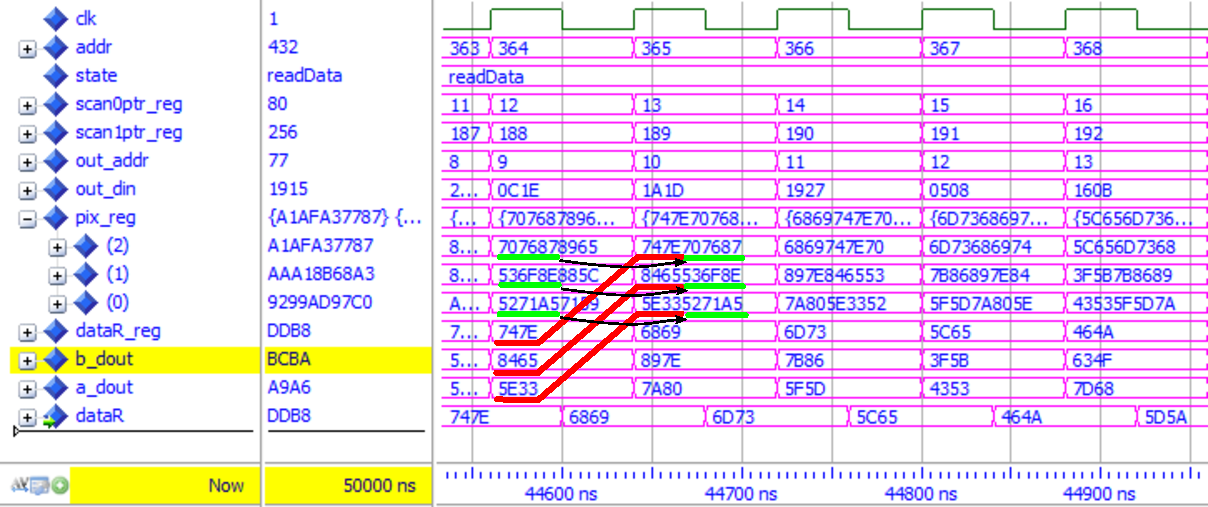
\includegraphics[width=0.8 \textwidth]{acc2_scan_annotated.pdf}
	\caption{Sliding window waveform (scanline version)}
	\label{fig:acc2_scanWaveSlide}
\end{figure}

\section{Burst mode access to external RAM}
\paragraph*{}
Initially we planned for an optimization that would exploit the synchronous mode of the external ram, to achieve the higher clock rate of $80MHz$. Some simulation result are acquired, but we have not been able to provide a working and verified burst mode implementation, within the time frame of this project. Appendix \ref{app:MemBurst} shows an attempt towards, simulating the external memory in continuous burst mode. The implementation consist of a small FSM that simulates the initial latency as well as the row boundary crossing delay that is described in the datasheet \cite{Micron:CellularRAM} of the external memory.
\paragraph*{}
Figure \ref{fig:burst_picture} shows the result obtained from a simulation run, the red markings indicates some of the visible errors in the processed image. The image seen in figure \ref{fig:pic_burst_err} is generated from the MATLAB verification script (app.\ref{app:Matlab}) and gives a more visible representation of the distribution of errors (the black color equals to no error, while the white color indicates an error). From the error image it is observed that the errors occurs systematically a at every $128word$. This gives a strong indication that there is a problem with the row boundary crossing, either in the memory simulation or in the accelerator code.  The burst mode optimization was expected to have a throughput close to $80M pix/sec$ but this is not confirmed, since the implementation has newer been tested in hardware.
     
\begin{figure}[H]
	\centering
	\begin{subfigure}[b]{0.5\textwidth}
		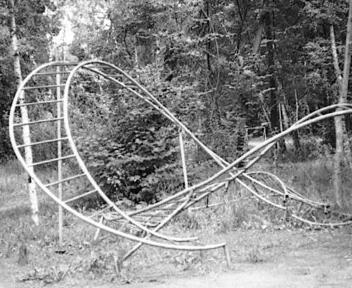
\includegraphics[width=1 \textwidth]{raw.png}
		\caption{Raw image before simulation}
		\label{fig:raw_burst}
    \end{subfigure}%
        ~ %add desired spacing between images, e. g. ~, \quad, \qquad, \hfill etc. 
    \begin{subfigure}[b]{0.5\textwidth}
    	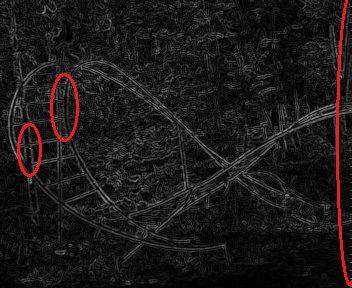
\includegraphics[width=1 \textwidth]{burstResult.png}
    	\caption{After simulation red blobs indicated errors}
    	\label{fig:burst_picture_sobel}
	\end{subfigure}
	\caption{Scanline buffering of pixel data.}
    	\label{fig:burst_picture}
\end{figure}


\begin{figure}[H]
	\centering
	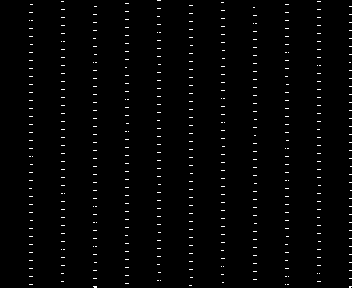
\includegraphics[width=0.5 \textwidth]{burstErr.png}
	\caption{Image of burst optimization errors}
	\label{fig:pic_burst_err}
\end{figure}